

%%%%%%%%%%%%%% 特徴量工学の説明 %%%%%%%%%%%%
\section{ニューラルネットワーク}
ニューラルネットワークは近年、``深層学習''あるいは``ディープラーニング''の名の元に、
再注目を浴びている学習モデルである。ニューラルネットワークは元々脳の神経活動を模倣したモデルとして
提案されたが、現在では学習の力学特性や統計物理学の知見など数理的な解析が行われている\cite{ディープローカルミニマム,DeepvsShallow}。
あるいはヒューリスティクスによる発展が著しい。
従って、本論文では単にある特定の形式で表される数理モデルとしてニューラルネットワークを扱う。

% ニューラルネットワークはパラメータ\(W\)を持つ層\(Layer(\cdot,W)\)と
% パラメータを持たない変換\(f(\cdot)\)によって構成されている。
% 層と変換を用いて作られたパラメトリックな合成関数をニューラルネットワークと呼ぶ。
% ニューラルネットワークを構成することで、BCIの候補となる関数族を決めることができるが、
% 裏を返すと、BCIとしての振る舞いができるようなニューラルネットワークの構成を選ばなければ、
% 学習を長時間続けたとしても良い結果は得られない。
\subsection{モデル構築と学習}
ニューラルネットワークは

\subsection{ニューラルネットワークに用いられる層}
\subsubsection{Linear層}
ニューラルネットワークで最も基本的な層はLinear層である。
Linear層はパラメータとして\(W \in \mathbb R^{d\times D}\)と\(b \in \mathbb R^d\)を有した
以下の関数である。
\begin{equation}
    L(x,W) = Wx + b
\end{equation}
% \begin{equation}
%     L(x,W) = \{Wx + b \mid W \in \mathbb R^{d\times D}, b \in \mathbb R^d\}
% \end{equation}
% Linear層は入力\(x\in R^D\)を\(d\)次元ベクトルへアフィン変換する。
% ここでLinear層の出力を\(y = Wx+b\)を成分表示をすると、
入力\(x=(x_1,\cdots,x_D)^T\)として、出力\(y=(y_1,\cdots,y_d)^T\)を以下で表すことができる。
\begin{equation}
    y_j = \sum_{i=1}^D  w_{j,i}x_i + b_j 
\end{equation}
ここに\(w_{j,i}\)は行列\(W\)の\((j,i)\)成分、\(b_j\)はベクトル\(b\)の\(j\)番目の成分である。
% 以下、層のパラメトリックな関数による記述と出力の成分表示にいずれの表記も場面に応じて使い分ける。

\subsubsection{Bilinear層}
Bilinear層は入力として\(x^{(1)}\in \mathbb R^{D_1}\)と\(x^{(2)}\in \mathbb R^{D_2}\)の
2つを受け取り、1つの出力\(y \in \mathbb R^d\)を返す。
\begin{equation}
    y_k = \sum_{j=1}^{D_1}\sum_{i=1}^{D_2}w_{j,i,k}x_j^{(1)}x_i^{(2)} + b_k
\end{equation}
ここでn階のテンソル\(A\in \mathbb R^{D_1,\cdots ,D_n}\)の\((d_1,\cdots,d_n)\)成分を\(a_{d_1,\cdots,d_n}\)と表記している。
パラメータは\(W\in \mathbb R^{D_1\times D_2 \times K}\)と\(b \in \mathbb R^K\)である。

\subsubsection{Convolution層}
Convolution層はパラメータとして\(H \in \mathbb R^{P\times Q\times C\times L}\)と\(B \in \mathbb R^{I\times J\times L}\)を有し、
入力を\(X \in \mathbb R^{I\times J\times C}\)として、出力\(Y \in \mathbb R^{I'\times J'\times L}\)は以下で表される。
\begin{equation}
    y_{i,j,l} = \sum_{c=1}^C \sum_{p=0}^{P-1} \sum_{q=0}^{Q-1}x_{i+p,j+q,c}h_{p,q,c,l}+b_{i,j,l}
    \label{eq:convlayer}
\end{equation}
ここでもn階のテンソル\(A\in \mathbb R^{D_1,\cdots ,D_n}\)の\((d_1,\cdots,d_n)\)成分を\(a_{d_1,\cdots,d_n}\)と表記している。
出力テンソルの大きさを決める\(I',J'\)は\(I,J\)と\(P,Q\)に依存し、それぞれ\(I'=P-I+1\)と\(J'=Q-J+1\)となる。
しかし、Convolution層は実応用ではstrideやpadding、dilationなどのテクニックによって更に複雑な動作をする。
これらのテクニックはそれぞれハイパーパラメータを持ち、\(I',J'\)はその全てに依存する。
% Convolution層については\(X*H=\sum_{p=0}^{P-1} \sum_{q=0}^{Q-1}x_{i+p,j+q,c}h_{p,q,c,l}\)と置き、(\ref{eq:convlayer})を以下の関数のように略記する。
% \begin{equation}
%     C(X,H) = \sum_{c} X*H + B
%     \label{eq:convlayer2}
% \end{equation}

\subsubsection{Recurrent層}
Recurrent層は入力\(X = (x_1,\cdots,x_T)\in \mathbb R^{D \times T}\)、
出力\(Y = (y_1,\cdots,y_T)\in \mathbb R^{d \times T}\)として以下で表される。
\begin{equation}
    y_t = {\rm tanh}(W_{in}x_t + W_{out}y_{t-1} + b) 
    \label{eq:reccurent}
\end{equation}
ここにパラメータは\(W_{in} \in \mathbb R^{d \times D}\)と\(W_{out} \in \mathbb R^{d \times d}\)ならびに、\(b \in \mathbb R^d \)である。
元々系列データへの応用のために考案されたため、
\(D\)次元のベクトル\(x_t \in \mathbb R^D\)が時間変化していくような場合を想定して
(\ref{eq:reccurent})と定式化される。
しかし、実際には入力は画像のような静的なデータでも構わなく、
画像を左から右に走査するような働きを担う。
\(\rm tanh(\cdot)\)は双曲線正接関数であるが、ニューラルネットワークの活性化関数として広く持ちいられている。

\subsubsection{LSTM層}
LSTMはLong Short-Term Memoryの略であり、
LSTM層はReccurent層が長期的な系列データを上手く学習できない問題を解決した。
LSTM層は入力\(X = (x_1,\cdots,x_T)\in \mathbb R^{D \times T}\)、
出力\(Y = (y_1,\cdots,y_T)\in \mathbb R^{d \times T}\)として以下で表される。
\begin{eqnarray}
    i_t &=& \sigma(W_{ii}x_t + W_{hi} h_{t-1} + b_i) \\
    f_t &=& \sigma(W_{if}x_t + W_{hf} h_{t-1} + b_f) \\
    o_t &=& \sigma(W_{io}x_t + W_{ho} h_{t-1} + b_o) \\
    g_t &=& {\rm tanh}(W_{ig}x_t + W_{hg} h_{t-1} + b_g) \\
    c_t &=& f_t \odot c_{t-1} + i_t \odot g_t \\
    y_t &=& o_t \odot {\rm tanh}(c_t)
    \label{eq:LSTM}
\end{eqnarray}
ここに\(\odot\)は同じ次元のベクトルの要素ごとの積である。
パラメータは\(W_{ii},W_{if},W_{io},W_{ig} \in \mathbb R^{d\times D}\)と、
\(W_{hi},W_{hf},W_{ho},W_{hg} \in \mathbb R^{d\times d}\)および、
\(b_{i},b_{f},b_{o},b_{g} \in \mathbb R^d\)である。
Recurrent層同様に、系列データを想定した定式化がなされているが、実際には入力が画像でも構わない。
\(\sigma(\cdot)\)はシグモイド関数であり(\ref{eq:logisticmodel})と同じものである。
ここでのシグモイド関数は、値域が\((0,1)\)であるために用いられている。

\(i_t,f_t,o_t,g_t\)は現在の入力\(x_t\)と過去の出力\(y_{t-1}\)を引数に取り、
それぞれ個別のパラメータを用いて値が算出される。
\(c_t\)はMemory Cellと呼ばれ、過去の情報を層の内部に記憶する役割を担っている。
\(f_t \in (0,1)^d \)を乗じることで、過去の情報\(c_{t-1}\)を一定の割合のみ保持し(あるいは忘却し)、
\(i_t\)に対して\(g_t \in (-1,1)^d\)を乗じた値を新たに加算して保持する。
\(y_t\)は内部情報である\(c_t\)を\((-1,1)^d\)にスケーリングしたベクトルと\(o_t\)との要素積によって算出される。
すなわち、\(o_t\)の値が内部情報\(c_t\)に応じて大きさと正負が調整されてLSTM層の出力となる。

\subsection{活性化関数}
ここではパラメータを持たない変換について述べる。
現在は数多くの活性化関数が利用されており、ここでまとめて扱う。
\subsubsection{シグモイド関数}
シグモイド関数\(\sigma(x)\)は以下で定義される。
\begin{equation}
    \sigma(z) = \frac{1}{1+\exp(-z)}
\end{equation}

ニューラルネットワークは当初、神経活動の数理モデルとしての一面を有しており、
入力値がある閾値を超えると発火するというモデルを表現するためにステップ関数が利用されていた。
シグモイド関数は、ステップ関数を微分可能な形で表現することを動機に考案された。

\subsubsection{双曲線正接関数}
双曲線正接関数\({\rm tanh}(z)\)は以下で定義される。
\begin{equation}
    {\rm tanh}(z) = \frac{\exp(z) - \exp(-z)}{\exp(z)+\exp(-z)}
\end{equation}
先に述べたシグモイド関数とは\(\sigma(z)=({\rm tanh}(x/2) + 1)/2\)という関係にあり、
負の値を取ることもできるため状況に応じてシグモイド関数の代わりに用いられる。

\subsubsection{ランプ関数}
ランプ関数はニューラルネットワークではRectified Linear Unit(ReLU)関数と呼ばれ、以下で表される。
\begin{equation}
    {\rm ReLU}(z) = \max(z,0)
\end{equation}
入力が正で\(-1\)の勾配を持ち、その他の場合は勾配は\(0\)となる。
この性質がニューラルネットワークの勾配消失問題を大きく改善したとされる。

\subsubsection{leaklyReLU関数}
ReLU関数が入力が負の場合にも値を有するように提案された。
\begin{equation}
    {\rm leaklyReLU}(z) = \max(z,0) + \alpha \min(z,0)
\end{equation}
入力が正で\(-1\)の勾配を持ち、その他の場合は勾配は\(\alpha\)でハイパーパラメータである。

\subsubsection{elu関数}
ReLU関数を全域で微分可能にするように調整された関数。
\begin{equation}
    {\rm elu}(z) = \max(z,0) + \min(\alpha(\exp(z)-1), 0)
\end{equation}
図\ref{fig:activation}はここまでに述べた5つの活性化関数の入出力を表した図である。
どのような場面でどの活性化関数が有効であるか、理論的な根拠は確認されておらず、
試行錯誤的に決定される。
\begin{figure}
    \centering
    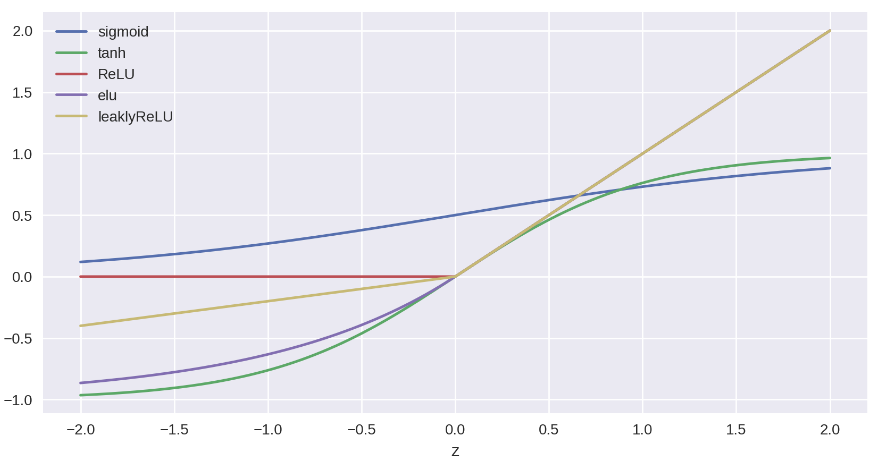
\includegraphics[width=14cm]{images/activations.png}
    \caption{5つの活性化関数}
    \label{fig:activation}
\end{figure}

\subsubsection{ソフトマックス関数}
ソフトマックス関数は一般的に、分類問題におけるニューラルネットワークの出力層に用いられる。
ベクトルの入力を受け取りベクトルの出力を行うが、以下に要素毎の計算を示す。
\begin{equation}
   {\rm softmax}_i(z) = \frac{\exp(z_i)}{\sum_j \exp(z_j)} 
\end{equation}
ここで、\(z_i\)はベクトル\(z\)の\(i\)番目の要素である。
定義から明らかに、値域は\((0,1)\)に制限され、出力の要素の総和は\(1\)である。

\subsection{過学習抑制手法}
\subsubsection{ドロップアウト}
ドロップアウトは過学習抑制のために考案された手法であり、以下で表される。
\begin{eqnarray}
    {\rm dropout}(z,p) & = & z \odot b \\
    b  & \sim & {\rm Bern}(p)
\end{eqnarray}
\({\rm Bern}(p)\)は\(p\)の確率で\(1\)を出力し、\(1-p\)の確率で\(0\)を出力するベルヌーイ分布である。
従って、ドロップアウトは入力\(z\)の各要素は\(1-p\)の確率で値を\(0\)に変更する。
ドロップアウトは入力が行われる度に毎回変更されるため、
学習時にはドロップアウトされなかった一部の要素に関わるパラメータのみが更新される。
テスト時にはドロップアウトを行わず、代わりに\(zp\)を出力する。
あるいはドロップアウトを用いたまま複数回サンプリングを行い、加算平均を出力とする。

パラメータを持つ全ての層の後にドロップアウトを適用した場合は、
ニューラルネットワークの学習がある仮定の下での変分ベイズ学習に厳密に一致する。
また、テスト時に複数回のサンプリングによる出力を行った場合、ベイズ予測分布に一致する\cite{ベイズドロップアウト}。
ただし、ベイズの解釈としては出力が確率的に\(0\)になるのではなく、学習パラメータが確率的に\(0\)になった結果、
出力が\(0\)になると考えなければならない。

\subsubsection{バッチ正規化}